\chapter{Linear Models for Regression}
\label{ch:regression}

\chapterguide%
  {\chapref{ch:supervised}, \chapref{ch:training}, and vectors/matrices from \chapref{ch:linear-algebra}.}
  {fit and interpret linear regression, diagnose residuals, engineer nonlinear terms, and regularize coefficients.}

Linear regression makes capacity, regularization, and optimization explicit. Through \chapref{ch:svm}, compare model families under the same workflow.

\section{The model}

Linear regression predicts a continuous value using a weighted sum of features:
\[
  \hat{y}=\beta_0+\beta_1x_1+\cdots+\beta_{p}x_{p}.
\]
$\beta_0$ predicts at zero-valued features; $\beta_j$ is the prediction change per unit of $x_j$, holding other features fixed.

\section{Least squares: how the line is chosen}

Ordinary least squares (OLS) chooses coefficients that minimize the residual sum of squares:
\[
  \min_{\bm{\beta}}
  \sum_{i=1}^{n}{(y_i-\hat{y}_i)}^2.
\]
A \term{residual}, $y_i-\hat y_i$, is the observed minus predicted value.

\begin{mlfigure}
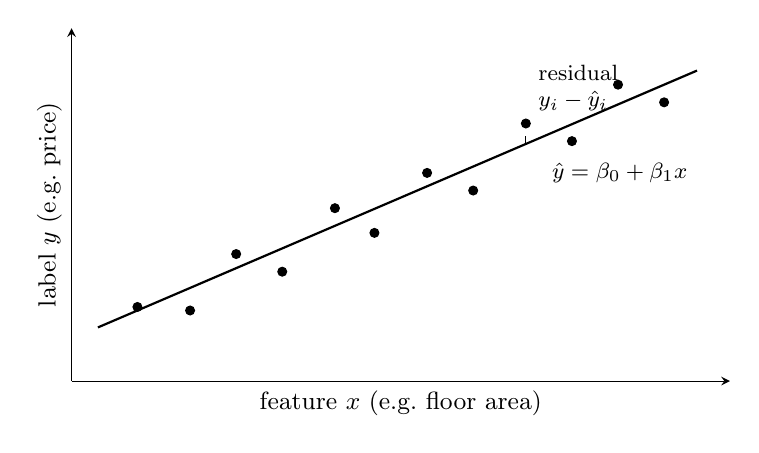
\begin{tikzpicture}
\begin{axis}[
  width=0.82\linewidth, height=0.50\linewidth,
  axis lines=left,
  xlabel={feature $x$ (e.g.\ floor area)},
  ylabel={label $y$ (e.g.\ price)},
  label style={font=\small},
  ticks=none, xmin=0, xmax=10, ymin=0, ymax=10,
  clip=false
]
\addplot[only marks, mark=*, mark size=1.6pt] coordinates {
  (1,2.1) (1.8,2.0) (2.5,3.6) (3.2,3.1) (4.0,4.9)
  (4.6,4.2) (5.4,5.9) (6.1,5.4) (6.9,7.3) (7.6,6.8)
  (8.3,8.4) (9.0,7.9)
};
\addplot[thick, domain=0.4:9.5] {0.8*x + 1.2};
\draw[dashed] (axis cs:6.9,6.72) -- (axis cs:6.9,7.3)
  node[above right=1pt, font=\footnotesize, align=left]
    {residual\\$y_i-\hat{y}_i$};
\node[font=\footnotesize, anchor=east]
  at (axis cs:9.5,5.9) {$\hat{y}=\beta_0+\beta_1 x$};
\end{axis}
\end{tikzpicture}
\end{mlfigure}

\begin{intuition}
Imagine rubber bands pulling observations toward the line. Least squares minimizes their total squared vertical lengths.
\end{intuition}

With a single feature, the best-fitting slope and intercept have simple closed forms:
\[
  \hat{\beta}_1
  =\frac{\sum_{i=1}^{n}(x_i-\bar{x})(y_i-\bar{y})}
        {\sum_{i=1}^{n}{(x_i-\bar{x})}^2},
  \qquad
  \hat{\beta}_0=\bar{y}-\hat{\beta}_1\bar{x}.
\]
Slope is covariance divided by feature variance. The intercept makes the line pass through $(\bar x,\bar y)$.

\begin{workedexample}
Fit a line to three points by hand: $(1,2)$, $(2,3)$, $(3,5)$.
The means are $\bar{x}=2$ and $\bar{y}=10/3$. The deviations from the means are $(-1,0,1)$ for $x$ and $(-\tfrac{4}{3},-\tfrac{1}{3},\tfrac{5}{3})$ for $y$. Then
\[
  \hat{\beta}_1
  =\frac{(-1)(-\tfrac{4}{3})+(0)(-\tfrac{1}{3})+(1)(\tfrac{5}{3})}
        {{(-1)}^2+0^2+1^2}
  =\frac{3}{2}=1.5,
  \qquad
  \hat{\beta}_0=\tfrac{10}{3}-1.5\times 2=\tfrac{1}{3}\approx 0.33.
\]
The fitted line is $\hat{y}=0.33+1.5x$, giving predictions $1.83$, $3.33$, and $4.83$ with residuals $+0.17$, $-0.33$, and $+0.17$. The residuals sum to zero --- a general property of least squares with an intercept.
\end{workedexample}

\section{Many features: the matrix view}

With the intercept absorbed into a leading column of ones in the design matrix $X\in\mathbb{R}^{n\times(p+1)}$, the objective and its gradient are
\[
  J(\bm{\beta})=\frac{1}{n}\|X\bm{\beta}-\bm{y}\|_2^2,
  \qquad
  \nabla_{\bm{\beta}}J
  =\frac{2}{n}X^{\mathsf T}(X\bm{\beta}-\bm{y}).
\]
Setting the gradient to zero gives the \term{normal equations} $X^{\mathsf T}X\bm{\beta}=X^{\mathsf T}\bm{y}$, whose solution (when $X^{\mathsf T}X$ is invertible) is
\[
  \hat{\bm{\beta}}={(X^{\mathsf T}X)}^{-1}X^{\mathsf T}\bm{y}.
\]
Solve the linear system with a stable factorization, or use gradient descent for large datasets. Explicit inversion is a teaching device, not the usual numerical approach.

\subsection{Reading the coefficients honestly}

\begin{itemize}
  \item Coefficients are in the label's units per unit of the feature, so their sizes are not comparable unless the features are standardized first.
  \item \term{Multicollinearity}: correlated features make individual coefficients unstable, even when predictions remain accurate.
  \item Coefficients are associations, not causal effects (\secref{sec:correlation}); adding or removing one feature can change the sign of another coefficient.
\end{itemize}

\subsection{The assumptions, in plain words}

Classical OLS assumptions include linearity in the chosen features, independent errors, constant error variance, and no exact collinearity. Violations can undermine coefficient interpretation and uncertainty estimates; inspect residuals for warning signs.

\section{Reading residuals: the diagnostic that matters most}

Inspect residuals $y-\hat y$ for structure the fitted model missed.

\begin{mlfigure}
\begin{tikzpicture}[baseline=(current bounding box.north)]
\begin{axis}[
  width=0.46\linewidth, height=4.1cm, axis lines=left,
  title style={font=\small\bfseries\color{MLGreen}}, title={Healthy: a formless cloud},
  xlabel={Prediction $\hat y$}, ylabel={Residual},
  label style={font=\scriptsize\color{MLMuted}}, tick label style={font=\scriptsize\color{MLMuted}},
  xmin=0, xmax=10, ymin=-3, ymax=3
]
\addplot[only marks,mark=*,mark size=1.2pt,MLGreen] coordinates {
(0.6,0.7)(1.2,-0.9)(1.8,0.3)(2.4,-1.4)(3.0,1.1)(3.6,-0.4)(4.2,1.6)(4.8,-1.1)
(5.4,0.2)(6.0,-1.7)(6.6,1.3)(7.2,-0.6)(7.8,0.9)(8.4,-1.2)(9.0,0.5)(9.5,-0.3)};
\draw[MLNavy,thick,dashed] (axis cs:0,0) -- (axis cs:10,0);
\end{axis}
\end{tikzpicture}
\hfill
\begin{tikzpicture}[baseline=(current bounding box.north)]
\begin{axis}[
  width=0.46\linewidth, height=4.1cm, axis lines=left,
  title style={font=\small\bfseries\color{MLRed}}, title={Sick: an obvious curve},
  xlabel={Prediction $\hat y$}, ylabel={Residual},
  label style={font=\scriptsize\color{MLMuted}}, tick label style={font=\scriptsize\color{MLMuted}},
  xmin=0, xmax=10, ymin=-3, ymax=3
]
\addplot[only marks,mark=*,mark size=1.2pt,MLRed] coordinates {
(0.6,2.1)(1.2,1.4)(1.8,0.6)(2.4,0.1)(3.0,-0.6)(3.6,-1.2)(4.2,-1.6)(4.8,-1.9)
(5.4,-1.8)(6.0,-1.5)(6.6,-1.0)(7.2,-0.3)(7.8,0.5)(8.4,1.3)(9.0,2.0)(9.5,2.5)};
\draw[MLNavy,thick,dashed] (axis cs:0,0) -- (axis cs:10,0);
\end{axis}
\end{tikzpicture}
\end{mlfigure}

\begin{keyidea}
Residual patterns suggest missing structure: curvature suggests nonlinear terms; a widening funnel suggests unequal error variance. Lab~2's insurance bands motivate a smoker $\times$ BMI interaction.
\end{keyidea}

\section{Polynomial regression: curves from a linear model}

Linear models are linear \emph{in parameters}. Adding $x^2$, $x^3$, or $x_1x_2$ allows curved predictions:
\[
  \hat{y}=\beta_0+\beta_1x+\beta_2x^2+\cdots+\beta_dx^d.
\]
Polynomial degree $d$ controls capacity; excessive degree can fit noise.

\begin{mlfigure}
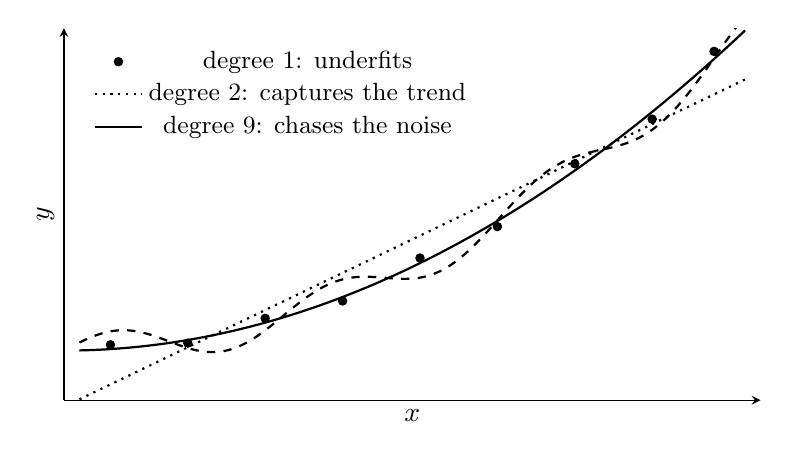
\begin{tikzpicture}
\begin{axis}[
  width=0.86\linewidth, height=0.52\linewidth,
  axis lines=left,
  xlabel={$x$}, ylabel={$y$},
  ticks=none, xmin=0, xmax=4.5, ymin=-3, ymax=19.5,
  legend style={draw=none, font=\small, at={(0.03,0.97)}, anchor=north west},
  clip=true
]
\addplot[only marks, mark=*, mark size=1.5pt] coordinates {
  (0.3,0.35) (0.8,0.45) (1.3,1.95) (1.8,3.0) (2.3,5.6)
  (2.8,7.5) (3.3,11.3) (3.8,14.0) (4.2,18.1)
};
\addplot[thick, dotted, domain=0.1:4.4, samples=60] {4.5*x-3.4};
\addlegendentry{degree 1: underfits}
\addplot[thick, domain=0.1:4.4, samples=80] {x^2};
\addlegendentry{degree 2: captures the trend}
\addplot[thick, dashed, domain=0.1:4.4, samples=160] {x^2 + 1.1*sin(deg(4.5*x))};
\addlegendentry{degree 9: chases the noise}
\end{axis}
\end{tikzpicture}
\end{mlfigure}

\begin{intuition}
Low degree may underfit; high degree may interpolate noise. Select degree using validation, not training fit.
\end{intuition}

Polynomial feature counts grow quickly, motivating regularization.

\section{Ridge regression: shrink everything a little}

\term{Ridge regression} adds an $L_2$ penalty on coefficient size to the least-squares objective. For centered features and label (so the intercept has been removed), its solution is
\[
  \hat{\bm{\beta}}_{\mathrm{ridge}}
  =\argmin_{\bm{\beta}}
  \|X\bm{\beta}-\bm{y}\|_2^2
  +\lambda\|\bm{\beta}\|_2^2
  ={(X^{\mathsf T}X+\lambda I)}^{-1}X^{\mathsf T}\bm{y}.
\]
The penalty trades fit against coefficient size. At $\lambda=0$, ridge is OLS; increasing $\lambda$ shrinks penalized coefficients. For $\lambda>0$, the centered system is invertible. Software usually leaves the intercept unpenalized and recovers it from the means.

\section{Lasso: shrink some coefficients to exactly zero}

\term{Lasso regression} swaps the penalty for an $L_1$ norm:
\[
  \hat{\bm{\beta}}_{\mathrm{lasso}}
  =\argmin_{\bm{\beta}}
  \|X\bm{\beta}-\bm{y}\|_2^2
  +\lambda\|\bm{\beta}\|_1.
\]
Lasso sets some coefficients exactly to zero, producing sparse models. Among strongly correlated features, however, it may choose one somewhat arbitrarily.

\subsection{Why the penalties behave differently}

Regularization constrains a coefficient budget. Least-squares contours touch an $L_1$ diamond often at axis corners, where coefficients are zero; an $L_2$ disk has no such corners.

\begin{mlfigure}
\begin{tikzpicture}[x=0.92cm, y=0.92cm, font=\small]
% ---- lasso panel ----
\begin{scope}
\draw[-{Stealth[length=2mm]}] (-1.5,0) -- (3.6,0) node[below] {$\beta_1$};
\draw[-{Stealth[length=2mm]}] (0,-1.1) -- (0,2.2);
\node[left] at (0,1.9) {$\beta_2$};
\draw[thick, fill=gray!18] (1,0) -- (0,1) -- (-1,0) -- (0,-1) -- cycle;
\draw[rotate around={39:(2.1,0.9)}] (2.1,0.9) ellipse (0.52 and 0.25);
\draw[rotate around={39:(2.1,0.9)}] (2.1,0.9) ellipse (0.95 and 0.45);
\draw[rotate around={39:(2.1,0.9)}] (2.1,0.9) ellipse (1.42 and 0.67);
\fill (2.1,0.9) circle (1.6pt) node[above right=0pt] {OLS fit};
\fill (1,0) circle (2pt);
\node[anchor=north, align=center, font=\footnotesize]
  at (1,-1.22) {lasso fit: $\beta_2=0$};
\node[anchor=west] at (0.35,2.65) {$L_1$ budget (diamond)};
\end{scope}
% ---- ridge panel ----
\begin{scope}[xshift=6.0cm]
\draw[-{Stealth[length=2mm]}] (-1.5,0) -- (3.6,0) node[below] {$\beta_1$};
\draw[-{Stealth[length=2mm]}] (0,-1.1) -- (0,2.2);
\node[left] at (0,1.9) {$\beta_2$};
\draw[thick, fill=gray!18] (0,0) circle (1);
\draw[rotate around={39:(2.1,0.9)}] (2.1,0.9) ellipse (0.52 and 0.25);
\draw[rotate around={39:(2.1,0.9)}] (2.1,0.9) ellipse (0.95 and 0.45);
\draw[rotate around={39:(2.1,0.9)}] (2.1,0.9) ellipse (1.35 and 0.64);
\fill (2.1,0.9) circle (1.6pt) node[above right=0pt] {OLS fit};
\fill (0.98,0.19) circle (2pt);
\node[anchor=north, align=center, font=\footnotesize]
  at (1,-1.22) {ridge fit: both small, neither zero};
\node[anchor=west] at (0.35,2.65) {$L_2$ budget (disk)};
\end{scope}
\end{tikzpicture}
\end{mlfigure}

\begin{intuition}
Regularization pulls coefficients toward zero: ridge shrinks them smoothly, while lasso can remove them entirely.
\end{intuition}

\section{Elastic net and practical guidance}

\term{Elastic net} combines both penalties,
\[
  \lambda\!\left(
  \rho\,\|\bm{\beta}\|_1
  +(1-\rho)\,\|\bm{\beta}\|_2^2
  \right),
\]
gaining lasso's sparsity while sharing weight across correlated features like ridge. The mixing parameter $\rho$ and strength $\lambda$ are both tuned on validation data.

Working habits that apply to every model in this chapter:

\begin{itemize}
  \item \term{Standardize features} so penalties act on comparable scales. Usually leave the intercept unpenalized.
  \item \term{Tune $\lambda$ with cross-validation} (\chapref{ch:evaluation}), searching over a logarithmic grid such as $10^{-3}$, $10^{-2}$, \ldots, $10^{2}$.
  \item \term{Starting choices:} ridge for many small effects; lasso for sparsity; elastic net for correlated groups.
  \item Consider \term{Huber loss} when extreme residuals dominate squared-error fitting.
\end{itemize}

\begin{keyidea}
A weighted-sum model, richer features, and a validated complexity penalty form a reusable modeling pattern.
\end{keyidea}

\begin{modelcard}{Linear Regression Family - Quick Guide}
\begin{tabularx}{\linewidth}{@{}>{\bfseries\leavevmode\color{MLNavy}}p{0.24\linewidth}X@{}}
Best when & The label is numerical, a weighted-sum relationship is a useful approximation, and interpretability matters. \cr
Start with & Ordinary linear regression, residual plots, and a mean/median baseline. \cr
Preprocessing & Encode categories; standardize before ridge, lasso, or elastic net; inspect skew and outliers. \cr
Main controls & Polynomial degree, regularization strength $\lambda$, and elastic-net mixing parameter. \cr
Watch for & Nonlinearity, influential outliers, multicollinearity, leakage, and unsafe extrapolation beyond the training range. \cr
\end{tabularx}
\end{modelcard}

\section{When ordinary squared error is the wrong model for the label}
\label{sec:special-regression-labels}

Use a different loss or distribution when the label structure or decision warrants it, not merely to make the model more elaborate.

\begin{mltable}
\begin{tabularx}{\linewidth}{@{}p{0.22\linewidth}p{0.29\linewidth}X@{}}
\toprule
\rowcolor{MLPaleBlue!92}
Label structure & Useful starting point & Main caution \\
\midrule
Continuous values with occasional large errors & Robust regression loss & Robustness changes which errors receive the most influence; validate against the real evaluation objective. \\
Conditional quantiles matter & Quantile regression & Different quantiles answer different questions and should not be interpreted as conditional means. \\
Non-negative counts & Count-aware generalized linear model & The chosen distributional assumptions must be plausible for the observed mean--variance relationship. \\
Positively skewed outcomes & Log-scale modeling or an appropriate positive-response model & Back-transformation changes the interpretation of average predictions and errors. \\
\bottomrule
\end{tabularx}
\end{mltable}

Validate specialized losses against the task metric and check prediction plausibility (\chapref{ch:evaluation}).

\begin{quickcheck}
\begin{enumerate}
  \item What does a regression coefficient mean when the other modeled features are held fixed, and why is that not automatically a causal effect?
  \item How do ridge and lasso change coefficient estimates differently as regularization becomes stronger?
  \item How can an interaction or polynomial feature let a model remain linear in its parameters while representing a nonlinear relationship in the original inputs?
\end{enumerate}
\end{quickcheck}